\begin{frame}[parent={concept:functional-testing}, hasprev=false, hasnext=true]
\frametitle{Cause-effect graph}
\label{concept:case-effect-graph}

\begin{block:concept}{Cause-effect graph}
Cause-effect graph establishes test requirements based on the possible
combinations of input conditions.
\end{block:concept}


\begin{block:fact}{Input conditions combination}
\begin{itemize}
	\item You could combine and select input conditions and test such
	combinations using equivalence partition.

	\item However, as the number of possible combinations is usually high,
	it is likely that the subsets of combinations to be tested will be chosen
	arbitrarily.
	\begin{itemize}
		\item This would lead to an ineffective test.
	\end{itemize}

	\item Cause-effect graphing aids in selecting, in a systematic way,
	a high yield set of test cases~\cite[p.~66]{Myers:2004}.
\end{itemize}
\end{block:fact}
\end{frame}


\begin{frame}[hasprev=true, hasnext=true]
\frametitle{Cause-effect graph}

\begin{block:fact}{Cause-effect graph}
\begin{itemize}
	\item The cause-effect graph creates a boolean graph that is a formal
	language to describe the software specification.
\end{itemize}
\end{block:fact}


\begin{block:fact}{Cause}
\begin{itemize}
	\item In the cause-effect graph, the causes corresponds to:
	\begin{itemize}
		\item input conditions of a given equivalence classes,
		\item stimulus,
		\item or anything else that causes an output of the program under
		testing.
	\end{itemize}
\end{itemize}
\end{block:fact}


\begin{block:fact}{Effect}
\begin{itemize}
	\item In the cause-effect graph, the effects are:
	\begin{itemize}
		\item the output,
		\item system state changes, or
		\item any observable outcome.
	\end{itemize}
\end{itemize}
\end{block:fact}
\end{frame}


\begin{frame}
\frametitle{Cause-effect graph}

\begin{block:procedure}{How to create the graph}
\begin{enumerate}
	\item Identify the possible input conditions (causes) and the possible
	actions of the product (effects).
	\begin{itemize}
		\item Hint: equivalence classes are a cause.
		\item Associate an unique identifier for each cause and effect found
		(a numeric id is fine).
	\end{itemize}

	\item Build a cause-effect graph by relating causes with identified
	effects.

    \item Impossible cause-effect combinations must be annotated in the graph.
\end{enumerate}
\end{block:procedure}
\end{frame}


\begin{frame}
\frametitle{Cause-effect graph}

\begin{block:fact}{Cause-effect graph elements}
\begin{itemize}
	\item Each node in the graph represents a input condition (cause) and
	outcomes (effects).

	\item Each node can be assigned the value 0 or 1.
	\begin{itemize}
		\item 0 represents the ``absent'' state.
		\item 1 represents the ``present'' state.
	\end{itemize}

	\item The relationships between the nodes is represented using the
	functions:
	\begin{itemize}
		\item identity,
		\item not,
		\item or,
		\item and.
	\end{itemize}
\end{itemize}
\end{block:fact}
\end{frame}


\begin{frame}
\frametitle{Cause-effect graph}


\begin{columns}[t]
\column{.4\textwidth}
\begin{block:fact}{Unary boolean functions}
\begin{tabular}{l|c|c}
\textbf{Function}			& \textbf{A}	& \textbf{Result}\\\hline\hline
\multirow{2}{*}{Identity} 	& 0 			& 0\\
							& 1 			& 1\\\hline\hline
\multirow{2}{*}{Not}		& 0 			& 1\\
							& 1				& 0\\
\end{tabular}
\end{block:fact}

\qquad
\column{.5\textwidth}
\begin{block:fact}{N-ary boolean functions}
\begin{tabular}{l|c|c|c}
\textbf{Function}			& \textbf{A}	& \textbf{B}	& \textbf{Result}\\\hline\hline
\multirow{4}{*}{Or} 		& 0 			& 0				& 0\\
							& 0 			& 1				& 1\\
							& 1 			& 0				& 1\\
							& 1 			& 1				& 1\\\hline\hline
\multirow{4}{*}{And}		& 0 			& 0				& 0\\
							& 0 			& 1				& 0\\
							& 1 			& 0				& 0\\
							& 1 			& 1				& 1\\
\end{tabular}
\end{block:fact}
\end{columns}

\end{frame}



\begin{frame}
\frametitle{Cause-effect graph}

\begin{block}{Function symbols}
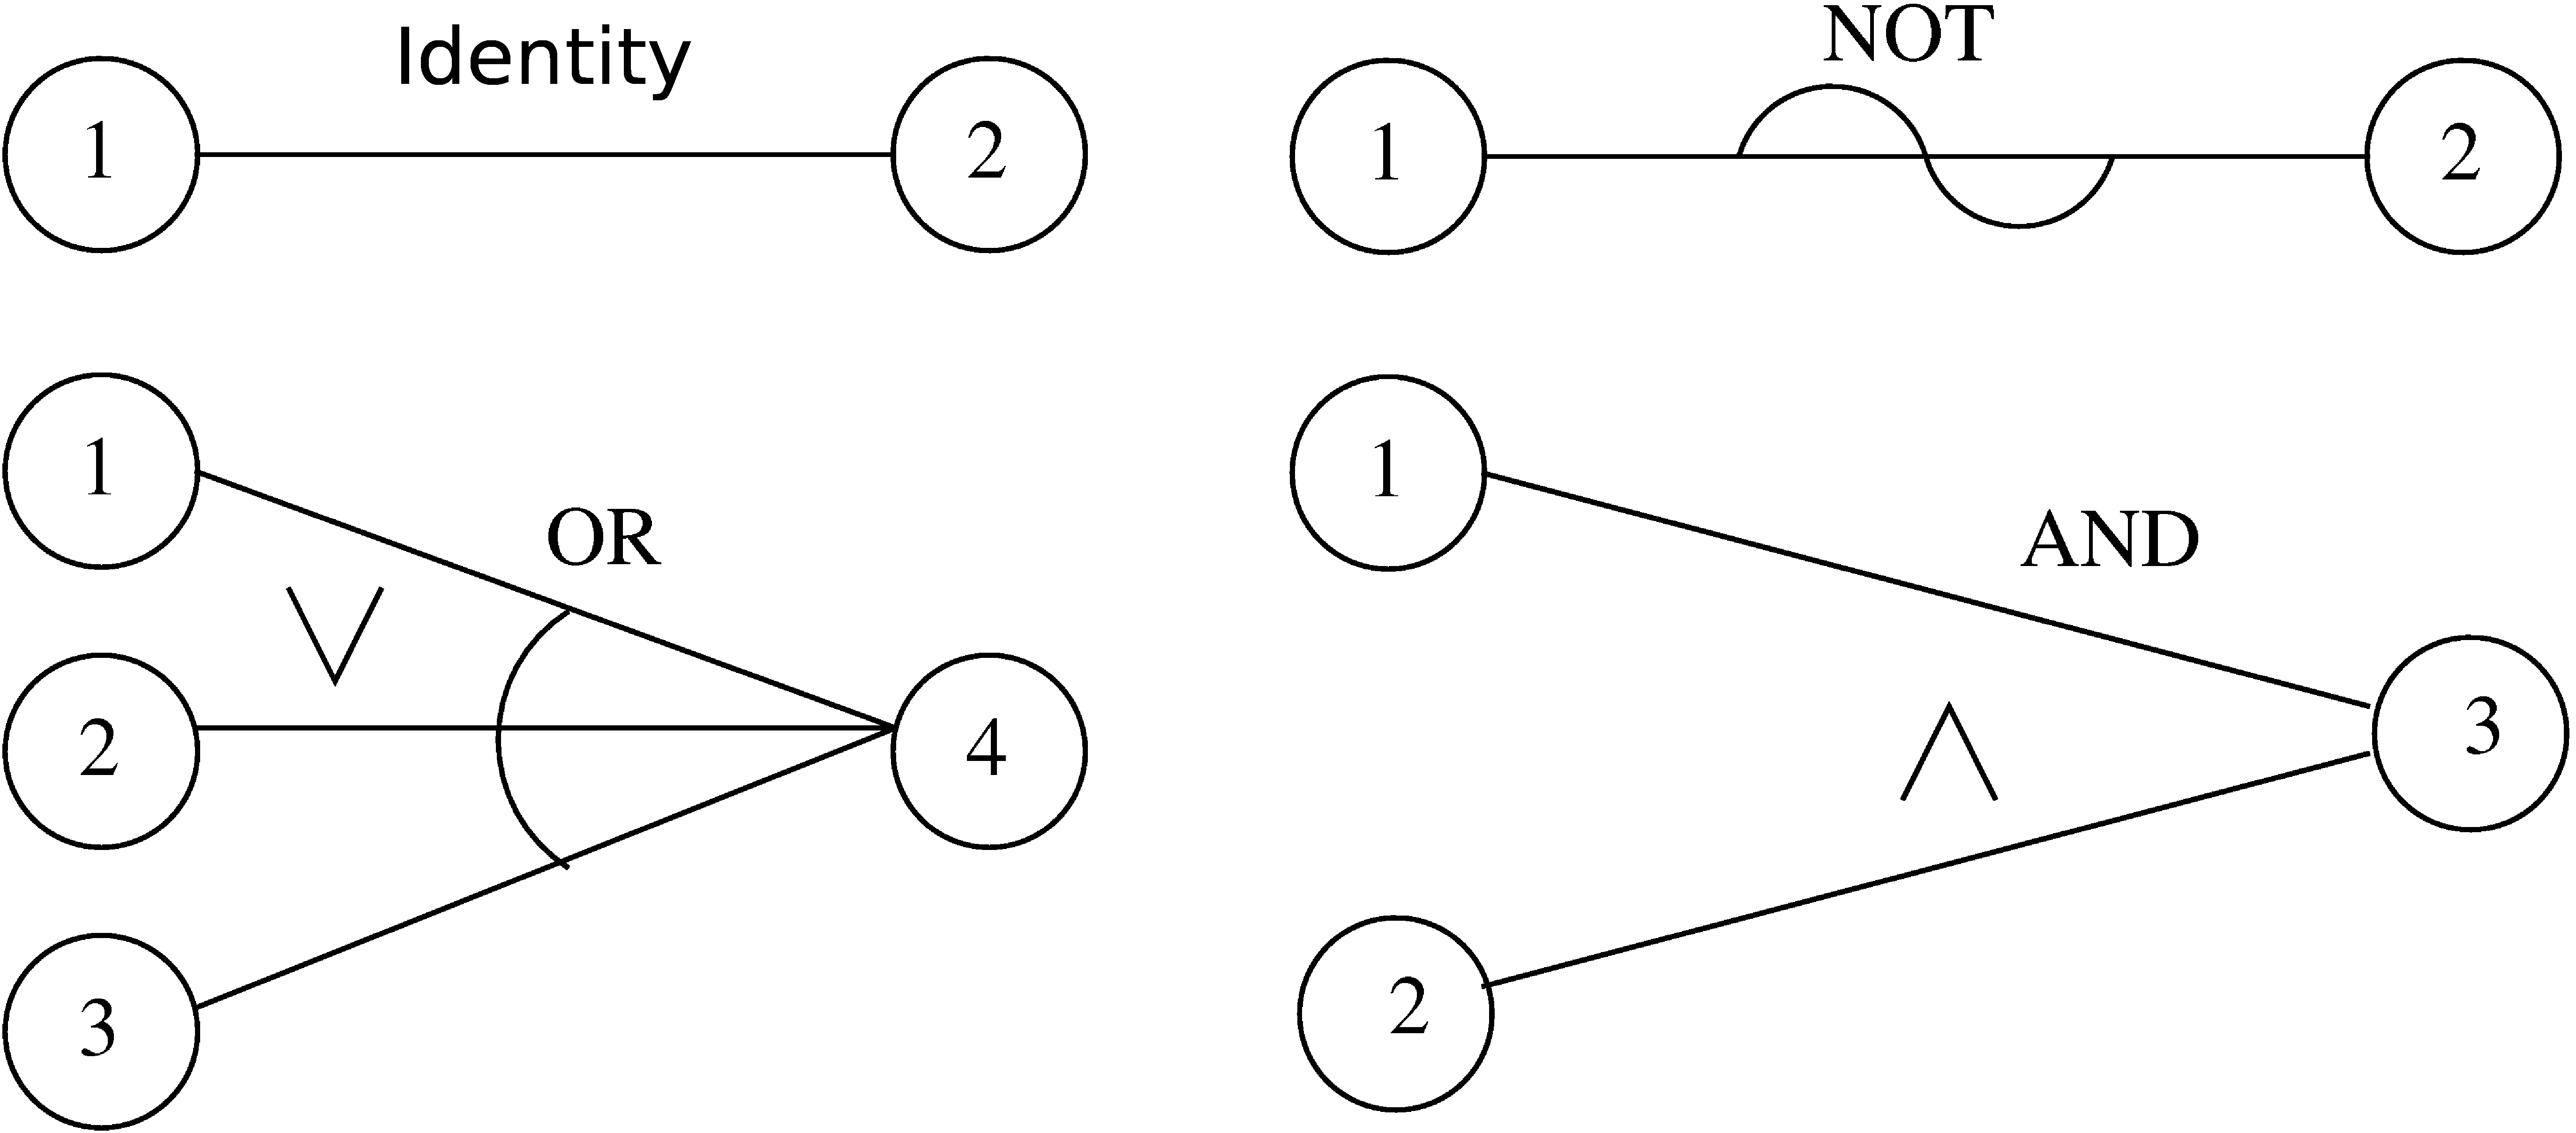
\includegraphics[scale=.04]{Functional testing/Cause-effect graph/Cause-effect graph symbols}
\end{block}

\begin{block}{Restrictions symbols}
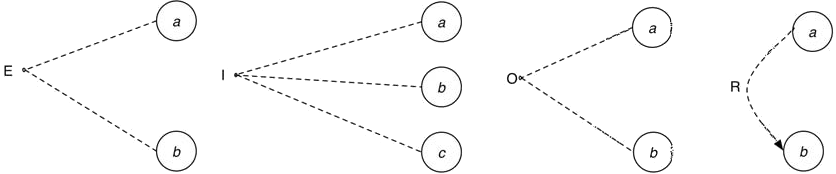
\includegraphics[width=\textwidth]{Functional testing/Cause-effect graph/Cause-effect graph restrictions}
\end{block}

\end{frame}





\begin{frame}
\frametitle{Cause-effect graph}
\label{procedure:cause-effect-graph}

\begin{block:procedure}{How to create the graph}
\begin{enumerate}
	\item To verify if the cause-effect graph is correct, it must be assigned
	the values 0 and 1 to the causes and check if the effects have the
	correct values.
\end{enumerate}
\end{block:procedure}


\hfill
\refie{example:cause-effect-graph}{\beamerbutton{Example}}
\end{frame}



\begin{frame}
\frametitle{Cause-effect graph}

\begin{block:procedure}{How to create the decision table}
\begin{enumerate}
	\item Convert the cause-effect graph into a decision table (from where test
	cases are derived).
	\begin{enumerate}
		\item Select an effect that should have the value 1.

		\item Trace back the cause-effect graph from the chosen effect, finding
		every cause combination that makes the effect have the value of 1.
		\begin{enumerate}
				\item In the cause-effect graph, if a node is of the OR-type
				and the output must be 1, never assign more than one input with
				the value 1 simultaneously.

				\item In the cause-effect graph, if a node is of the AND-type
				and the output must be 0, all the input combinations that
				returns an output of 0 must be enumerated. However, if one of
				the input is 0 and one or more of the input is 1, it is not
				necessary to enumerate all the conditions which input are
				equal to 1.
		\end{enumerate}
	\end{enumerate}
\end{enumerate}
\end{block:procedure}
\end{frame}


\begin{frame}
\frametitle{Cause-effect graph}

\begin{block:procedure}{How to create the decision table}
\begin{enumerate}
	\item (continuation) Convert the cause-effect graph into a decision table
	(from where test cases are derived).
	\begin{enumerate}
		\item Create a column in the decision table for every cause
		combination.

		\item Specify, for every cause combination, the state of every single
		effect, annotating them in the table.
	\end{enumerate}
\end{enumerate}
\end{block:procedure}
\end{frame}


% \begin{frame}[hasprev=true, hasnext=false]
% \frametitle{Cause-effect graph}
%
% \begin{block:fact}{}
% \begin{itemize}
% 	\item The definition of the cause-effect graph helps to point out
% 	incompleteness and ambiguities in the software requirement
% 	specification~\cite[p. 66]{myers:2004}.
% \end{itemize}
% \end{block:fact}
% \end{frame}

